\documentclass{standalone}
\usepackage{tikz}

\begin{document}
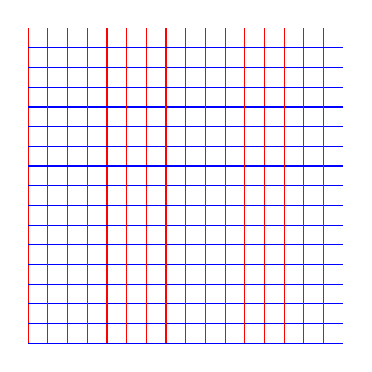
\begin{tikzpicture}[x=1cm, y=1cm]
    % Draw the white square
    \draw[white] (0,0) rectangle (4,4);

    % Draw red and blue lines in a crisscross pattern
    \foreach \i in {0, 0.5, 1, 1.5, 2, 2.5, 3, 3.5} {
        \draw[red] (\i,0) -- (\i,4);
        \draw[blue] (0,\i) -- (4,\i);
    }

    \foreach \i in {0.25, 0.75, 1.25, 1.75, 2.25, 2.75, 3.25, 3.75} {
        \draw[red] (\i,0) -- (\i,4);
        \draw[blue] (0,\i) -- (4,\i);
    }
\end{tikzpicture}
\end{document}